\chapter{Pruebas y resultados}
\label{chap:pruebas}

Este capítulo describe la estrategia de pruebas aplicada al sistema, las técnicas y herramientas utilizadas en cada nivel, los resultados obtenidos y las decisiones que se toman a partir de ellos. Se abordan cinco frentes: las pruebas automatizadas del código, las pruebas funcionales de extremo a extremo contra la infraestructura real, las pruebas de rendimiento asociadas a los requerimientos no funcionales, la evaluación del modelo de detección y la evaluación de usabilidad del \emph{dashboard}. Los resultados se presentan con las condiciones en que se obtienen, y se distingue lo medido de lo inferido.

\section{Estrategia de pruebas}
\label{sec:estrategia-pruebas}
La estrategia combina pruebas automatizadas, que se ejecutan en cada cambio del código, con verificaciones manuales y mediciones puntuales para los aspectos que dependen del sistema operativo, de los servicios externos o del comportamiento del modelo sobre datos reales. La tabla~\ref{tab:tecnicas-prueba} resume las técnicas aplicadas, la herramienta utilizada y el alcance de cada una.

\begin{longtable}{>{\raggedright\arraybackslash}p{3.3cm}>{\raggedright\arraybackslash}p{4.2cm}>{\raggedright\arraybackslash}p{6.6cm}}
	\caption{Técnicas de prueba, herramientas y alcance}
	\label{tab:tecnicas-prueba}\\
	\hline
	\textbf{Técnica} & \textbf{Herramienta} & \textbf{Alcance} \\
	\hline
	\endfirsthead
	\hline
	\textbf{Técnica} & \textbf{Herramienta} & \textbf{Alcance} \\
	\hline
	\endhead
	Pruebas unitarias & pytest & Reglas del motor de \emph{scoring} (decaimiento, niveles, regla de piso), proveedores IAM, notificaciones, respaldo de modelos y componentes del agente (colectores, \emph{buffer}, \emph{circuit breaker}, reversión), con las dependencias del sistema operativo simuladas. \\
	\hline
	Pruebas de integración de la API & pytest, cliente de pruebas de FastAPI y Redis simulado en memoria & Endpoints de configuración, autenticación, auditoría, integración IAM y salud del servicio, sin servicios externos. \\
	\hline
	Pruebas de extremo a extremo del \emph{scoring} & pytest con los modelos entrenados & Evaluación de eventos completos con los modelos reales: período de aprendizaje, persistencia de la explicación y recarga de modelos sin reinicio. \\
	\hline
	Prueba automatizada de extremo a extremo PDP$\rightarrow$PEP & pytest con los modelos entrenados y el código real del agente & Ciclo completo entre el punto de decisión y el de aplicación, con los efectos sobre el sistema operativo reemplazados por un registro en memoria (sección~\ref{sec:pruebas-e2e}). \\
	\hline
	Medición de cobertura & coverage.py con pytest-cov & Cobertura de líneas y de ramas de la API y del agente, medida por separado (sección~\ref{sec:cobertura-codigo}). \\
	\hline
	Pruebas de contrato & pytest & Estructura del evento que el agente envía a la API, contrato de los endpoints de salud y validación de rangos de configuración. \\
	\hline
	Pruebas de regresión & Script propio de regresión & Comparación del puntaje calculado en línea contra el cálculo fuera de línea sobre historiales reales del conjunto de datos. \\
	\hline
	Análisis estático y compilación & oxlint, compilador de TypeScript, Vite y npm audit & Calidad, tipado, construcción y dependencias vulnerables del \emph{frontend}. \\
	\hline
	Integración continua & GitHub Actions & Ejecución automática de las suites, del análisis estático y de la validación de la infraestructura en cada \emph{push}. \\
	\hline
	Pruebas funcionales manuales & Scripts de demostración y ensayo & Escenarios de extremo a extremo contra Redis y PostgreSQL reales, incluida la ejecución de mitigaciones en el \emph{endpoint}. \\
	\hline
	Pruebas de rendimiento & Scripts de medición con requests y psutil & Latencia de evaluación de eventos (RNF-01) y consumo de recursos del agente (RNF-02). \\
	\hline
	Evaluación del modelo & Métricas no supervisadas, escenarios inyectados y escenarios etiquetados & Comportamiento del modelo híbrido sobre el conjunto de datos y sensibilidad ante escenarios de ataque simulados; detección y falsos positivos sobre escenarios con etiqueta conocida en una partición reservada (sección~\ref{sec:benchmark}). \\
	\hline
	Evaluación de usabilidad & Evaluación heurística & Interfaz del \emph{dashboard} contra las diez heurísticas de usabilidad de Nielsen. \\
	\hline
\end{longtable}

\section{Pruebas automatizadas}
\label{sec:pruebas-automatizadas}

Esta sección presenta el inventario de pruebas automatizadas, los resultados de su ejecución, la integración continua y la cobertura de los requerimientos.

\subsection{Inventario}
El repositorio contiene 530 pruebas automatizadas, 353 de la API y 177 del agente (algunas funciones de prueba se ejecutan con varios juegos de parámetros). La tabla~\ref{tab:inventario-pruebas} las agrupa por componente.

\begin{longtable}{>{\raggedright\arraybackslash}p{2.6cm}>{\raggedright\arraybackslash}p{1.9cm}>{\raggedright\arraybackslash}p{1.9cm}>{\raggedright\arraybackslash}p{7.5cm}}
	\caption{Inventario de pruebas automatizadas por componente}
	\label{tab:inventario-pruebas}\\
	\hline
	\textbf{Componente} & \textbf{Archivos} & \textbf{Pruebas} & \textbf{Tipos y foco} \\
	\hline
	\endfirsthead
	\hline
	\textbf{Componente} & \textbf{Archivos} & \textbf{Pruebas} & \textbf{Tipos y foco} \\
	\hline
	\endhead
	API de \emph{scoring} & 35 & 353 & Unitarias, de integración, de extremo a extremo con modelos reales, de contrato y de regresión. Cubren autenticación y sesiones, ligadura de las claves de agente, configuración y su atomicidad, auditoría, período de aprendizaje, explicación persistida, IAM, notificaciones con y sin el modelo de lenguaje, persistencia con una base de datos simulada, planificador de reentrenamiento y el ciclo PDP$\rightarrow$PEP, el criterio de promoción del modelo y la paridad de las variables entre versiones. \\
	\hline
	Agente local & 14 & 177 & Unitarias con el sistema operativo simulado: colectores, filtro de procesos, \emph{buffer} local, \emph{circuit breaker}, exigencia de HTTPS, confirmación de acciones, reversión de la ACL y contrato del evento. \\
	\hline
	\emph{Frontend} & -- & -- & Sin pruebas unitarias; se valida con análisis estático, verificación de tipos y compilación. \\
	\hline
\end{longtable}

\subsection{Resultados de la ejecución}
La tabla~\ref{tab:ejecucion-pruebas} presenta el resultado de la ejecución completa realizada el 10 de octubre de 2026, en un entorno aislado, sin servicios externos configurados y sin ejecución real de mitigaciones.

\begin{longtable}{>{\raggedright\arraybackslash}p{5.4cm}>{\raggedright\arraybackslash}p{8.4cm}}
	\caption{Resultados de la ejecución de las pruebas automatizadas}
	\label{tab:ejecucion-pruebas}\\
	\hline
	\textbf{Suite} & \textbf{Resultado} \\
	\hline
	\endfirsthead
	\hline
	\textbf{Suite} & \textbf{Resultado} \\
	\hline
	\endhead
	API, suite completa con los modelos entrenados & 353 aprobadas, 0 fallidas, 0 omitidas \\
	\hline
	API, configuración de integración continua (sin los modelos entrenados) & 326 aprobadas, 18 omitidas, 0 fallidas \\
	\hline
	Agente, suite completa en Windows & 177 aprobadas, 0 fallidas \\
	\hline
	\emph{Frontend}, análisis estático & Sin errores \\
	\hline
	\emph{Frontend}, compilación & Correcta, con una advertencia por el tamaño del paquete de la biblioteca de gráficos \\
	\hline
\end{longtable}

Las 18 pruebas omitidas en la configuración de integración continua dependen de artefactos que no están versionados: 15 requieren los modelos entrenados y 3 verifican la paridad de las variables con la segunda versión del modelo. La cobertura de código se mide y se informa en la sección~\ref{sec:cobertura-codigo}.

\subsection{Integración continua}\label{sec:integracion-continua}
El repositorio cuenta con un \emph{pipeline} de GitHub Actions que se ejecuta en cada \emph{push} y está compuesto por cuatro trabajos independientes:
\begin{itemize}
	\item \textbf{\emph{Frontend}} (Ubuntu, Node~24): análisis estático y compilación; no tiene umbral de cobertura, porque el \emph{frontend} no tiene pruebas.
	\item \textbf{API} (Ubuntu, Python~3.11): ejecución de las pruebas de la API sin los artefactos de modelo, que no están versionados, con medición de la cobertura combinada de líneas y ramas del código de la API y de los dos módulos auxiliares que importa. El umbral es del 74\,\% de cobertura combinada y funciona como protección contra regresiones. El mismo informe se publica además por líneas, solo a título informativo (sin umbral), y cuatro archivos de pruebas del agente que no dependen del sistema operativo se ejecutan allí sin medir cobertura y deben pasar.
	\item \textbf{Agente en Windows (\texttt{agent-windows}):} ejecución de la suite completa del agente en Windows (Python~3.11), con un umbral del 85\,\% de cobertura de líneas.
	\item \textbf{Infraestructura} (Ubuntu, Terraform~1.16.4): verificación de formato, inicialización y validación de la configuración sin aplicar cambios; sin umbral.
\end{itemize}

Una corrida del trabajo de la API falló porque faltaba la dependencia de lectura de archivos Parquet que usa el criterio de promoción; se agregó a los requisitos de la API. Con esa corrección, el \emph{pipeline} finaliza con los cuatro trabajos aprobados. La integración continua no ejecuta las pruebas que requieren artefactos de modelo no versionados (18 omitidas y cuatro archivos excluidos), entre ellas la prueba de extremo a extremo PDP$\rightarrow$PEP, ni la prueba de regresión. Esas suites se ejecutan localmente.

\subsection{Cobertura de código}\label{sec:cobertura-codigo}
La cobertura se mide con \emph{coverage.py} 7.16 (mediante \emph{pytest-cov} 7.1), con medición de ramas activada, sobre todo el código del producto que se ejecuta en operación:
\begin{itemize}
	\item el punto de decisión de políticas (PDP), es decir, el código de la API;
	\item los dos módulos auxiliares de \emph{scripts} que la API importa en ejecución;
	\item el punto de aplicación de políticas (PEP), es decir, el agente.
\end{itemize}
El alcance está versionado en el repositorio. Las únicas exclusiones son el envoltorio de ejecución del punto de entrada del agente y una función que solo usa un análisis fuera de línea. No se excluyó ningún módulo del producto por depender de servicios externos: la persistencia en PostgreSQL, el planificador de reentrenamiento, los colectores y la aplicación de acciones se prueban con dobles (un motor de base de datos simulado, subprocesos triviales, bibliotecas del sistema simuladas y carpetas temporales).

Cada componente se mide por separado con su propia suite: la API con los artefactos de modelo entrenados y el agente en Windows, su sistema operativo soportado. La evidencia del objetivo del 85\,\% es esta medición local completa, con artefactos, que se realiza con un \emph{script} del repositorio. El umbral se fija sobre la cobertura de líneas; la cobertura combinada de líneas y ramas se informa como dato adicional.

\begin{longtable}{>{\raggedright\arraybackslash}p{4.2cm}>{\raggedright\arraybackslash}p{1.9cm}>{\raggedright\arraybackslash}p{2.3cm}>{\raggedright\arraybackslash}p{1.9cm}>{\raggedright\arraybackslash}p{2.9cm}}
	\caption{Cobertura de código por componente}
	\label{tab:cobertura-codigo}\\
	\hline
	\textbf{Componente} & \textbf{Pruebas} & \textbf{Sentencias} & \textbf{\% líneas} & \textbf{\% líneas y ramas} \\
	\hline
	\endfirsthead
	\hline
	\textbf{Componente} & \textbf{Pruebas} & \textbf{Sentencias} & \textbf{\% líneas} & \textbf{\% líneas y ramas} \\
	\hline
	\endhead
	API (PDP) & 353 & 2\,469 & \textbf{93,9} & 92,4 \\
	\hline
	Agente (PEP) & 177 & 1\,116 & \textbf{89,3} & 88,1 \\
	\hline
	\textbf{Total} & \textbf{530} & 3\,585 & \textbf{92,5} & 91,1 \\
	\hline
\end{longtable}
{\small Fuente: elaboración propia.\par}

El informe de evidencia (HTML, XML y resumen) se genera con un \emph{script} del repositorio. En integración continua, el trabajo del agente en Windows exige el 85\,\% de líneas en cada \emph{push}. El trabajo de la API mide la cobertura sin los artefactos de modelo, que no están versionados: el núcleo de \emph{scoring} no se ejercita allí y el 74\,\% que exige funciona como protección contra regresiones, no como evidencia del objetivo; esa evidencia es la medición local completa.

Antes de agregar las pruebas de este ciclo, la misma suite daba 84,2\,\% de líneas en la API y 69,4\,\% en el agente. Con el criterio de promoción implementado y probado (RF-21), el módulo de métricas de la promoción de modelos alcanza el 98,8\,\% de líneas.

\textbf{\emph{Frontend}.} El \emph{dashboard} queda fuera del umbral, y se declara así explícitamente. Por una invariante de la arquitectura, el \emph{frontend} no contiene lógica de negocio: no calcula el puntaje, no aplica el decaimiento ni combina modelos. Solo muestra lo que expone la API y edita la configuración operativa, que la API valida. El riesgo funcional del sistema reside en la API y en el agente, que son los componentes medidos. El \emph{frontend} se valida con análisis estático y verificación de tipos en cada \emph{push}, y de forma manual contra la API.

\subsection{Cobertura de los requerimientos}
La tabla~\ref{tab:cobertura-requerimientos} relaciona los requerimientos del capítulo~\ref{chap:requerimientos} con el tipo de evidencia de prueba disponible.

\begin{longtable}{>{\raggedright\arraybackslash}p{4.4cm}>{\raggedright\arraybackslash}p{9.7cm}}
	\caption{Evidencia de prueba por requerimiento}
	\label{tab:cobertura-requerimientos}\\
	\hline
	\textbf{Evidencia} & \textbf{Requerimientos} \\
	\hline
	\endfirsthead
	\hline
	\textbf{Evidencia} & \textbf{Requerimientos} \\
	\hline
	\endhead
	Prueba automatizada & RF-01 a RF-07, RF-09 a RF-25, RF-27 a RF-31; RNF-03, RNF-04, RNF-06 a RNF-08 y RNF-11 \\
	\hline
	Prueba parcial & RF-26 (el campo que expone la API tiene prueba automatizada; el indicador del \emph{dashboard} se verifica en forma manual); RNF-05 (el \emph{buffer}, el reenvío y el \emph{circuit breaker} tienen prueba automatizada; el descarte por vencimiento y por tope se verifica en el código) \\
	\hline
	Verificación manual o medición & RF-08 (ejecución real de acciones en el \emph{endpoint}); RNF-01 y RNF-02 (mediciones de la sección~\ref{sec:pruebas-rendimiento}); RNF-09 (verificación de la cadena de \emph{hashes}); RNF-13 (TLS del despliegue; el rechazo de URLs \texttt{http} fuera de \emph{loopback} por el agente tiene prueba automatizada); RNF-10 (corrida real de reentrenamiento); RNF-12 (ejecución en Windows); RNF-14 (ensayos de concurrencia); RNF-15 (evaluación heurística) \\
	\hline
\end{longtable}

Los requerimientos con verificación manual o con prueba parcial se encuentran implementados y se verifican con las mediciones y ejecuciones documentadas en las secciones siguientes, que no forman parte de la suite automatizada.

\section{Pruebas funcionales de extremo a extremo}
\label{sec:pruebas-e2e}
Las pruebas automatizadas se ejecutan con Redis simulado y sin base de datos. La integración entre el punto de decisión (API) y el punto de aplicación (agente) se valida, además, con una prueba de extremo a extremo automatizada. La prueba reproduce el guion de la demostración en el mismo proceso: 46 eventos de calentamiento, exfiltración de archivos y salida por un país simulado. Usa el código real del agente para construir cada evento, interpretar el veredicto y confirmar la acción, y la API real con los modelos entrenados para decidir. Solo se reemplazan los efectos sobre el sistema operativo (terminar procesos y denegar la carpeta) por un registro en memoria. La prueba verifica cuatro puntos. Primero, que cada evento recibe puntaje, nivel y una acción coherente con la política configurada. Segundo, que el nivel escala hasta alto y crítico. Tercero, que en crítico el agente ejecuta la terminación y la denegación (esta última una sola vez). Cuarto, que la confirmación del agente queda registrada y expuesta por la API. Los eventos respetan la ventana temporal que la API exige (no más de 5 minutos en el futuro ni más de 90 días en el pasado), sin desactivarla. La misma secuencia está disponible como ensayo ejecutable antes de la demostración. La prueba requiere los artefactos de modelo, que no están versionados; por eso corre en el entorno local y no en la integración continua, donde se omite.

Para verificar el sistema contra la infraestructura real se realizan pruebas funcionales manuales, documentadas con su fecha y resultado:

\begin{itemize}
	\item \textbf{Demostración de seis escenas (agosto de 2026).} Se ejecutaron contra Redis y PostgreSQL reales seis escenarios que recorren el caso de uso CU-01 y el CU-02: un usuario de bajo riesgo, una exfiltración de archivos con mitigación en el \emph{endpoint}, una aplicación no monitoreada, el catálogo de acciones de mitigación, una conexión de red y la configuración de umbrales con un rechazo por validación. Cada corrida generó un reporte de auditoría automático.
	\item \textbf{Ensayo de la cadena de decisión.} Un script envía una secuencia de eventos de exfiltración y registra la evolución del nivel. En la última ejecución, el primer evento quedó en nivel medio, el nivel alto se alcanzó en el evento 15 y el crítico en el evento 44, con la acción correspondiente devuelta al agente en cada caso.
	\item \textbf{Período de aprendizaje (agosto y septiembre de 2026).} Contra la API conectada a los servicios reales, se verificó la lectura y modificación del umbral de aprendizaje, el rechazo de valores fuera de rango y la exigencia de autenticación de administrador.
	\item \textbf{Reentrenamiento y promoción (agosto de 2026).} Se verificó en vivo el reemplazo del modelo sin reiniciar la API cuando el modelo nuevo iguala al vigente y el rechazo cuando empeora. Además, una corrida real disparada por el planificador el 25 de agosto completó el \emph{pipeline} en aproximadamente 1~h~50~min y no promovió el modelo, porque el error de reconstrucción del LSTM empeoró de 0,1155 a 0,1175. Estas verificaciones corresponden al criterio de promoción anterior; el vigente se describe en la sección~\ref{sec:reentrenamiento-producto}.
	\item \textbf{Integridad de los eventos crudos (agosto de 2026).} La verificación de la cadena de \emph{hashes} sobre la tabla de eventos crudos resultó correcta en el 100\,\% de las filas, antes y después de registrar un evento nuevo.
	\item \textbf{Concurrencia (septiembre de 2026).} Con hasta 50 escrituras concurrentes sobre PostgreSQL no se produjeron errores, y el disparador que calcula la cadena de \emph{hashes} agregó en promedio 0,042~ms por inserción.
	\item \textbf{Concurrencia sobre Redis (agosto de 2026).} Contra el Redis gestionado, con hasta 15 escrituras simultáneas sobre el estado de un mismo usuario, entre 3 y 4 de cada 20 fallaban por conflicto de transacción. Con 20 reintentos y una espera aleatoria entre ellos, se completaron sin error 70 de 70 escrituras concurrentes. Este ensayo respalda RNF-14.
\end{itemize}

Como complemento, el código del agente, de la API y del \emph{frontend} se somete a revisiones estáticas de seguridad y mantenibilidad, con rondas de correcciones posteriores. La auditoría de dependencias del \emph{frontend} finalizó sin vulnerabilidades reportadas.

\section{Pruebas de rendimiento}
\label{sec:pruebas-rendimiento}

Esta sección evalúa dos requerimientos no funcionales de rendimiento: la latencia de evaluación de eventos (RNF-01) y el consumo de recursos del agente (RNF-02).

\subsection{Latencia de evaluación de eventos (RNF-01)}
Se mide la latencia de extremo a extremo de la evaluación de eventos desde el lado del cliente: 1000 eventos medidos, precedidos por 50 de calentamiento que se descartan, enviados en secuencia y distribuidos entre cinco usuarios con una mezcla de tipos representativa de la actividad que captura el agente. La API se ejecuta en el mismo equipo, con Redis en memoria y sin base de datos. La tabla~\ref{tab:rnf01} presenta los resultados.

\begin{longtable}{>{\raggedright\arraybackslash}p{6.0cm}>{\raggedright\arraybackslash}p{4.0cm}}
	\caption{Latencia de evaluación de eventos (RNF-01)}
	\label{tab:rnf01}\\
	\hline
	\textbf{Métrica} & \textbf{Valor} \\
	\hline
	\endfirsthead
	\hline
	\textbf{Métrica} & \textbf{Valor} \\
	\hline
	\endhead
	Media & 16,96~ms \\
	\hline
	Mediana & 13,35~ms \\
	\hline
	Percentil 95 & 14,91~ms \\
	\hline
	Percentil 99 & 148,87~ms \\
	\hline
	Máximo & 880,26~ms \\
	\hline
	Errores & 0 de 1000 \\
	\hline
	Rendimiento secuencial & 59 eventos por segundo \\
	\hline
\end{longtable}

El umbral fijado para RNF-01 es un percentil 95 menor o igual a 500~ms y un percentil 99 menor o igual a 1~s. El criterio se justifica porque el \emph{dashboard} consulta el estado cada 2~s y el agente captura actividad con una frecuencia del orden de un segundo: un evento evaluado en menos de medio segundo no se acumula. El resultado cumple el umbral con amplio margen.

Una segunda medición con el juego de modelos vigente, en otro equipo (Windows~11, procesador AMD de 16 núcleos lógicos), da un percentil 95 de 13,0~ms y un percentil 99 de 108,9~ms, con 1000 de 1000 eventos evaluados sin error, lo que confirma el cumplimiento del umbral.

Las latencias más altas coinciden con los eventos que completan una secuencia de 50 eventos de un usuario, que es cuando se ejecuta la inferencia del LSTM. Esta relación se infiere de la posición de los valores extremos y no está instrumentada. La medición tiene dos limitaciones: Redis en memoria no representa la latencia de red de un Redis gestionado, y los eventos se envían de forma secuencial, sin carga concurrente de varios agentes.

\subsection{Consumo de recursos del agente (RNF-02)}
Para RNF-02 se registra, cada 5~s durante 30 minutos de uso normal del equipo, el consumo de CPU del proceso del agente, normalizado sobre el total de núcleos lógicos, y su memoria residente. El agente se ejecuta en modo de simulación de mitigaciones, de modo que la medición refleja la captura y el envío de eventos sin efectos sobre el equipo. El umbral es un consumo medio de CPU menor o igual al 5\,\% de la máquina y una memoria residente menor o igual a 150~MB. La medición se realizó el 8 de octubre de 2026 en un equipo con Windows~11 Pro y 16 núcleos lógicos: se tomaron 360 muestras sin pérdidas y el agente envió unos 112 eventos, todos respondidos. La tabla~\ref{tab:rnf02} presenta los resultados.

\begin{longtable}{>{\raggedright\arraybackslash}p{4.0cm}>{\raggedright\arraybackslash}p{3.0cm}>{\raggedright\arraybackslash}p{3.0cm}>{\raggedright\arraybackslash}p{3.0cm}}
	\caption{Consumo de recursos del agente (RNF-02)}
	\label{tab:rnf02}\\
	\hline
	\textbf{Métrica} & \textbf{Media} & \textbf{Percentil 95} & \textbf{Máximo} \\
	\hline
	\endfirsthead
	\hline
	\textbf{Métrica} & \textbf{Media} & \textbf{Percentil 95} & \textbf{Máximo} \\
	\hline
	\endhead
	CPU (\% de la máquina) & 0,09 & 0,14 & 0,16 \\
	\hline
	Memoria residente (MB) & 33,02 & 33,24 & 33,25 \\
	\hline
\end{longtable}

El agente cumple el umbral con un margen amplio: su consumo medio de CPU es más de cincuenta veces menor que el límite y su memoria residente se mantiene estable durante toda la medición, cerca de un quinto del máximo admitido. La medición refleja el uso normal del equipo; no incluye una ráfaga de eventos de archivo como la del escenario de exfiltración, en la que el percentil 95 y el máximo podrían ser mayores.

\section{Evaluación del modelo sin etiquetas}
\label{sec:evaluacion-modelo}

Las métricas corresponden al juego de modelos vigente, entrenado en la corrida del 2 de septiembre de 2026 sobre CLUE-LDS (50.522.931 eventos; 8.494.616 tras la limpieza), con 27 eventos duplicados por reproducciones de prueba sin efecto práctico, y con las referencias de percentil regeneradas el 6 de octubre de 2026. La regla de promoción anterior rechazó ese juego por diferencias del orden del ruido; se adopta como vigente porque es el único juego completo y coherente (modelo, escaladores, codificación y referencias) disponible, y la evaluación de la sección~\ref{sec:benchmark} se realiza sobre él. La sección se organiza en dos partes: primero se fijan las metas de evaluación y se contrasta con ellas el resultado obtenido, y luego se presentan las métricas no supervisadas que describen el comportamiento del modelo híbrido y el acuerdo entre sus dos componentes.

\subsection{Metas de evaluación}\label{sec:metas-modelo}
El conjunto de datos CLUE-LDS no incluye etiquetas de actividad maliciosa
\parencite{Landauer2022Dataset}, por lo que la evaluación no puede expresarse en exactitud, precisión,
exhaustividad o F1. Una versión preliminar del trabajo planteaba un enfoque supervisado sobre
el conjunto de datos de autenticación de Los Alamos National Laboratory (LANL)
\parencite{Kent2015}, cuyas 253 sesiones anómalas, derivadas de los registros de un ejercicio de
red team sobre más de 7,6 millones de sesiones, exigían técnicas de balanceo de clases. Ese
enfoque se descarta al adoptar CLUE-LDS: las etiquetas de LANL corresponden a otro conjunto de
datos y a otra unidad de análisis (la sesión, no el usuario-día), y ninguna fase del
\emph{pipeline} vigente las utiliza. En su lugar, se fijan las metas de la tabla~\ref{tab:metas-modelo}, que combinan el
comportamiento del modelo sobre datos sin etiquetar con la detección de escenarios de ataque
inyectados (sección~\ref{sec:validacion-escenarios}).

\begin{table}[h]
\centering
\caption{Metas de evaluación del modelo y resultado obtenido}
\label{tab:metas-modelo}
\begin{tabular}{p{5.2cm}p{3.2cm}p{3cm}p{1.8cm}}
\hline
Métrica & Meta & Resultado & Cumple \\
\hline
Tasa de anomalías de Isolation Forest en prueba & entre 1\,\% y 3\,\% (contaminación del 2\,\%) & 0,81\,\% & No \\
Tasa de anomalías del LSTM en prueba & entre 3\,\% y 7\,\% (umbral en el percentil 95) & 4,18\,\% & Sí \\
Detección atribuible del escenario combinado (E4) con el umbral del nivel alto (70) & $\geq$ 50\,\% de los usuarios & 13,3\,\% (2 de 15) & No \\
Detección atribuible promedio de los cuatro escenarios con umbral 70 & $\geq$ 33\,\% & 5,0\,\% (3 de 60) & No \\
Usuario-días sin inyección que terminan en nivel alto o crítico & $\leq$ 10\,\% & 15,4\,\% & No \\
Latencia de evaluación, percentil 95 (RNF-01) & $\leq$ 500\,ms & 14,9\,ms & Sí \\
\hline
\end{tabular}\par
{\small Fuente: elaboración propia.\par}
\end{table}
\FloatBarrier

Las metas se fijan después de una primera evaluación exploratoria, en la que las de detección y de alertas tampoco se cumplían, y no se modifican al pasar al juego de modelos vigente; cualquier reentrenamiento posterior se informa contra estas mismas metas.

Las tasas de anomalías se comparan con el parámetro que cada modelo usa para fijar su umbral: una
tasa muy por debajo indica que el umbral es más estricto en prueba que en entrenamiento. La meta
de detección exige que al menos la mitad de los ataques combinados, que son los más evidentes,
lleven al usuario al nivel alto, y la meta de alertas acota la carga de revisión sobre actividad
normal a uno de cada diez usuario-días. Los resultados muestran que el sistema cumple las metas de
rendimiento y de comportamiento del LSTM, pero no las de detección ni de alertas: es la principal
limitación técnica del proyecto, cuyas causas se analizan en la sección~\ref{sec:interpretacion}.

\subsection{Métricas no supervisadas}\label{sec:metricas-no-supervisadas}
Como el conjunto de datos no incluye etiquetas de actividad maliciosa \parencite{Landauer2022Dataset}, no es posible calcular precisión, exhaustividad (\emph{recall}), F1 ni curvas ROC, que requieren conocer qué eventos corresponden a un ataque. La escasez de datos etiquetados es una limitación frecuente en la detección de anomalías sobre registros de actividad \parencite{Landauer2023Survey}. En su lugar, el modelo se evalúa con métricas de comportamiento y de acuerdo entre sus dos componentes, presentadas en la tabla~\ref{tab:metricas-modelo}, y con la validación por escenarios de la sección~\ref{sec:validacion-escenarios}. La sección~\ref{sec:benchmark} supera en parte esta limitación con escenarios de etiqueta conocida.

\begin{longtable}{>{\raggedright\arraybackslash}p{5.2cm}>{\raggedright\arraybackslash}p{3.4cm}>{\raggedright\arraybackslash}p{5.5cm}}
	\caption{Métricas no supervisadas del modelo híbrido}
	\label{tab:metricas-modelo}\\
	\hline
	\textbf{Métrica} & \textbf{Valor} & \textbf{Lectura} \\
	\hline
	\endfirsthead
	\hline
	\textbf{Métrica} & \textbf{Valor} & \textbf{Lectura} \\
	\hline
	\endhead
	Tasa de anomalías de Isolation Forest en prueba & 0,81\,\% (99 de 12\,236 usuario-días) & Inferior a la proporción de contaminación fijada en el entrenamiento (2\,\%). \\
	\hline
	Tasa de anomalías del LSTM Autoencoder en prueba & 4,18\,\% (1\,558 de 37\,254 secuencias) & Cercana al 5\,\% esperable por usar el percentil 95 del error como umbral. \\
	\hline
	Error de reconstrucción del LSTM & Media 0,1225; umbral 0,1180 & Umbral definido como el percentil 95 del error en entrenamiento. \\
	\hline
	Distribución del puntaje híbrido & Mediana 42,0; percentil 95 69,3; percentil 99 82,8 & La mayor parte de la actividad queda por debajo del umbral del nivel alto (70). \\
	\hline
	Correlación entre modelos & $-0{,}22$ (Pearson; 234 usuarios con cobertura completa, $p < 0{,}001$) & Correlación débil y negativa: los modelos capturan aspectos distintos del comportamiento. \\
	\hline
	Coincidencia de anomalías & Índice de Jaccard 0,111 (6 usuarios marcados por ambos modelos) & Las anomalías que marca cada modelo casi no se superponen. \\
	\hline
\end{longtable}

La correlación se calcula sobre los 234 usuarios con cobertura de ambos modelos, porque los conjuntos de prueba de cada modelo solo comparten 15 usuarios; restringida a esos 15, la correlación es $r = -0{,}41$ ($p = 0{,}13$, no significativa). La baja coincidencia indica que los dos modelos no son redundantes, lo que es consistente con la decisión de combinarlos. Sin embargo, estas métricas no demuestran que la combinación detecte mejor que cada modelo por separado, y el peso de 0,5 asignado a cada uno no tiene un respaldo cuantitativo. Además, los conjuntos de prueba de los dos modelos se construyen con criterios distintos (partición temporal para Isolation Forest y por usuario para el LSTM), por lo que la comparación entre ambos es limitada.

\section{Validación por escenarios inyectados}
\label{sec:validacion-escenarios}

Esta sección describe el método de validación mediante escenarios inyectados, sus resultados, la sensibilidad de la detección según el umbral y la interpretación de los resultados.

\subsection{Método}
Para obtener una medida de la capacidad de detección sin etiquetas, se inyectan escenarios de ataque sintéticos sobre historiales reales. Se seleccionan al azar, con semilla fija, 15 usuarios del período de prueba con entre 50 y 4000 eventos y al menos cinco días de actividad. Para cada usuario se reproduce su historial completo a través de la API, se toma una instantánea del estado y, a partir de ella, se inyecta cada escenario por separado, restaurando el estado entre uno y otro:
\begin{itemize}
	\item \textbf{E1, exfiltración:} entre 30 y 60 eventos de creación y escritura de archivos, uno cada 5~s, en horario laboral y desde el país habitual.
	\item \textbf{E2, fuera de horario:} hasta 40 eventos reales del último día de actividad, reubicados entre las 2 y las 5 de la mañana.
	\item \textbf{E3, cambio de país:} los mismos eventos, en su horario original, informados desde otro país.
	\item \textbf{E4, combinado:} la exfiltración de E1 en horario nocturno y desde otro país.
\end{itemize}

Se considera \emph{detección atribuible} a la inyección que lleva el nivel del usuario a alto o crítico cuando antes de inyectar estaba por debajo de alto. Así se descartan los usuarios que ya se encontraban en nivel alto por el riesgo acumulado. Como referencia de alertas sobre actividad presuntamente legítima, se registra el nivel de cierre de cada día del período de prueba sin inyección (650 usuario-días).

\subsection{Resultados}
La tabla~\ref{tab:escenarios} presenta los resultados con la política vigente, en la que el nivel alto comienza en un puntaje de 70 y el crítico en 90.

\begin{longtable}{>{\raggedright\arraybackslash}p{3.2cm}>{\raggedright\arraybackslash}p{2.3cm}>{\raggedright\arraybackslash}p{2.3cm}>{\raggedright\arraybackslash}p{2.3cm}>{\raggedright\arraybackslash}p{2.0cm}}
	\caption{Resultados de la validación por escenarios (15 usuarios por escenario)}
	\label{tab:escenarios}\\
	\hline
	\textbf{Escenario} & \textbf{Alto o crítico} & \textbf{Ya en alto antes} & \textbf{Atribuibles} & \textbf{Crítico} \\
	\hline
	\endfirsthead
	\hline
	\textbf{Escenario} & \textbf{Alto o crítico} & \textbf{Ya en alto antes} & \textbf{Atribuibles} & \textbf{Crítico} \\
	\hline
	\endhead
	E1, exfiltración & 2 & 2 & 0 & 0 \\
	\hline
	E2, fuera de horario & 3 & 2 & 1 & 0 \\
	\hline
	E3, cambio de país & 2 & 2 & 0 & 0 \\
	\hline
	E4, combinado & 4 & 2 & 2 & 0 \\
	\hline
\end{longtable}

Sobre los días sin inyección, el 15,4\,\% de los usuario-días (100 de 650) terminó en nivel alto y ninguno en crítico. La proporción fue del 14,3\,\% (79 de 553) para los días con cobertura completa de ambos modelos y del 21,6\,\% (21 de 97) para los días con cobertura parcial, y se concentró en los usuarios con pocos días de historial. Estas proporciones corresponden al nivel de cierre del día (alto o superior), que incluye la regla de piso: con el puntaje numérico de cierre y el umbral de 70, la proporción es del 14,2\,\% en total (12,8\,\% con cobertura completa y 21,6\,\% con cobertura parcial). Los 8 días de diferencia son de cobertura completa, en los que un modelo marcó anomalía y la regla de piso elevó el nivel.

Las inyecciones elevaron la mediana del puntaje entre 3,5 y 5,6 puntos respecto del valor previo, pero el puntaje máximo mediano de cada escenario quedó entre 63,5 y 65,6, por debajo del umbral del nivel alto. Las tres detecciones atribuibles corresponden a dos usuarios con cobertura completa (Isolation Forest y LSTM): \texttt{civilian-gray-weasel-garagemanager} en el escenario combinado (de 64,4 a 70,6) y \texttt{vivacious-aquamarine-prawn-streettrader} en los escenarios fuera de horario y combinado (de 68,8 a 72,9 y a 72,8). Las tres cruzan apenas el límite del nivel alto (70), sin regla de piso, y se explican solo por variables de Isolation Forest. Todas las explicaciones generadas provinieron de las variables de Isolation Forest (proporción de actividad fuera de horario, hora promedio y entropía de tipos de evento); en 7 de los 60 casos ninguna variable superó el umbral de explicación.

\subsection{Sensibilidad según el umbral}
Para analizar el compromiso entre sensibilidad y alertas sobre actividad normal sin modificar la configuración del sistema, se recalcula la detección atribuible para umbrales entre 40 y 90. La figura~\ref{fig:curva-umbral} muestra el resultado.

\begin{figure}[ht]
	\centering
	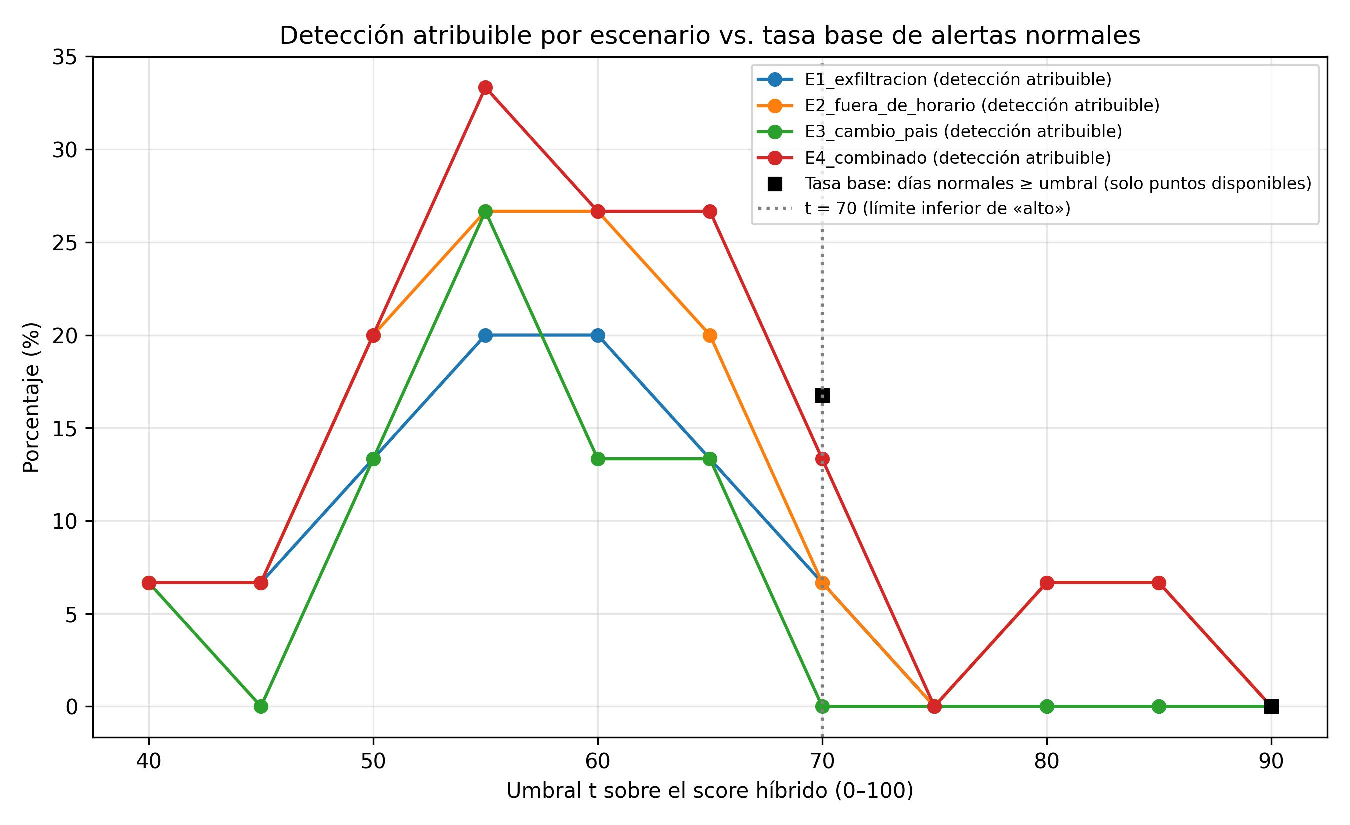
\includegraphics[width=\textwidth]{images/pruebas/curva_umbral.pdf}
	\caption{Detección atribuible por escenario según el umbral, y tasa de alertas sobre días sin inyección (porcentaje de usuario-días) para umbrales entre 40 y 90}
	\label{fig:curva-umbral}
	{\small Fuente: elaboración propia.\par}
\end{figure}

La detección atribuible alcanza su máximo en la zona de 55 a 65 puntos, con un 33,3\,\% para el escenario combinado en los umbrales de 55 y de 65, y nunca supera un tercio de los usuarios. La curva no es monótona porque, al bajar el umbral, una proporción creciente de usuarios ya lo supera antes de la inyección: en el umbral de 40, el 93,3\,\% de los usuarios parte por encima, mientras que en el de 70 lo hace solo el 13,3\,\%. Con el puntaje de cierre de cada día, la tasa de días sin inyección que superan el umbral cae de 98,9\,\% con un umbral de 40 a 71,1\,\% con 55, 26,3\,\% con 65, 14,2\,\% con 70 y 0\,\% con 90. En la zona de 55 a 65, donde la detección atribuible alcanza su máximo (33,3\,\% en el escenario combinado), entre una cuarta parte y dos tercios de los días normales también superarían el umbral. En ningún umbral la detección atribuible supera con claridad a la tasa de alertas sobre días normales. Con el nivel de cierre, que incluye la regla de piso, la tasa en el umbral de 70 es del 15,4\,\%.

\subsection{Interpretación}
\label{sec:interpretacion}
Con la política vigente, el sistema detecta pocos de los escenarios inyectados y ninguno alcanza el nivel crítico, de modo que la mitigación más severa no se dispara ante estos ataques simulados. Esto es consistente con una política conservadora, que reserva la terminación de procesos y la denegación de acceso para el nivel crítico, pero también indica una sensibilidad baja ante ataques de corta duración.

Entre las causas, varias están verificadas. El 99,95\,\% de los eventos del conjunto de datos tiene el país registrado como desconocido, por lo que la variable de cambio de país casi no varía durante el entrenamiento. Esto explica que el escenario E3 no se detecte y, a la vez, que cuando esa variable cambia domine el error de reconstrucción del LSTM. Además, el LSTM no aprovecha el orden de los eventos: permutar los 50 eventos de una secuencia no cambia el ordenamiento. Su riesgo correlaciona $-0{,}68$ con el logaritmo del volumen de actividad del usuario, de modo que tiende a marcar a los usuarios poco activos. Las demás causas son inferidas y no se aíslan experimentalmente:
\begin{itemize}
	\item Isolation Forest trabaja con variables agregadas por día, en las que una ráfaga de 30 a 60 eventos no resulta atípica para un usuario con un historial variable.
	\item El LSTM evalúa secuencias de 50 eventos, por lo que una inyección corta completa a lo sumo una secuencia y su señal se diluye.
	\item La combinación con la línea base personal y el decaimiento temporal amortiguan los cambios puntuales; en el caso del decaimiento, el benchmark confirma que empeora el ordenamiento en ventanas cortas (sección~\ref{sec:decisiones-pruebas}).
\end{itemize}

La alta proporción de alertas en usuarios con pocos días de historial es consistente con el sesgo conocido del componente de riesgo personal en usuarios con historial escaso. Los resultados deben leerse con cautela: se trata de 15 usuarios por escenario, con una sola inyección por caso, escenarios diseñados por el propio equipo y una referencia de normalidad sin verificación. Una diferencia de un usuario equivale a 6,7 puntos porcentuales.

\section{Evaluación con escenarios etiquetados}
\label{sec:benchmark}
La validación de la sección~\ref{sec:validacion-escenarios} utiliza 15 usuarios y una sola inyección por caso. Esta sección la amplía con un conjunto mayor de víctimas, escenarios con etiqueta conocida, una partición que separa los experimentos de la evaluación final e intervalos de confianza. Con etiquetas construidas de este modo es posible calcular sobre el sistema en producción las métricas que la ausencia de etiquetas impide obtener sobre los datos originales: el área bajo la curva ROC, la exhaustividad (\emph{recall}) y la tasa de falsos positivos.

\subsection{Escenarios}
Como CLUE-LDS no incluye ataques, los escenarios se construyen sobre el historial real de cada víctima a partir de un instante T. La tabla~\ref{tab:bench-escenarios} los describe.

\begin{table}[h]
\centering
\caption{Escenarios del benchmark de detección}
\label{tab:bench-escenarios}
\begin{tabular}{>{\raggedright\arraybackslash}p{3.0cm}>{\raggedright\arraybackslash}p{2.6cm}>{\raggedright\arraybackslash}p{8.8cm}}
\hline
Escenario & Qué simula & Construcción \\
\hline
S1 similar y S1 disímil & Toma de cuenta & Desde el instante T, los eventos de la víctima en una ventana de 7 días se reemplazan por los de otro usuario activo en la misma ventana: el más parecido (similar) o el menos parecido (disímil), según una similitud que pondera con 0,3 el cociente de eventos por día y con 0,7 el índice de Jaccard de los tipos de evento. \\
\hline
S2, con $k$ = 2, 5 y 10 & Exfiltración & En cada día activo de la ventana se inyecta una ráfaga de eventos de archivo y de compartición de $k$ veces la mediana diaria de eventos de archivo de la víctima, en una hora habitual para ella. \\
\hline
S2 solo archivos, con $k$ = 10 & Exfiltración sin compartir & Igual que S2, pero solo con eventos de archivo, para separar el efecto de la compartición. \\
\hline
S3 & Uso fuera de horario & Los eventos de cada día se reubican entre las 2 y las 5 de la mañana, hora de Viena, conservando su orden. \\
\hline
\end{tabular}\par
{\small Fuente: elaboración propia a partir del benchmark de detección.\par}
\end{table}
\FloatBarrier

Cada escenario se construye en dos versiones. En la versión sin país, los eventos conservan su ubicación original, desconocida en casi todos los casos, por lo que el escenario mide el comportamiento; en la versión con país, los eventos modificados llevan un país atacante, lo que mide el efecto de la ubicación sobre los modelos. El escenario S1 reproduce la fórmula y los pesos de similitud de la herramienta publicada por los autores del conjunto de datos \parencite{Landauer2022Dataset}, con cuatro diferencias: se toman los extremos de similitud en lugar de pares al azar, el reemplazo es unidireccional, la etiqueta se asigna por usuario-día dentro de la ventana y los usuarios donantes se restringen a los que el LSTM no vio en su entrenamiento.

\subsection{Partición y métricas}
Se toman como víctimas los 123 usuarios con al menos 5 días activos posteriores al corte temporal de Isolation Forest (2 de agosto de 2021), repartidos por estrato de actividad previa en dos particiones: DEV, con 63 víctimas, y HOLDOUT, con 60. Con al menos una ventana válida para los escenarios quedan 62 y 57, respectivamente. Todos los experimentos con variantes del cálculo del puntaje se realizan solo sobre DEV, y HOLDOUT se utiliza una única vez, para la evaluación final que presenta esta sección. Isolation Forest se entrena con una partición temporal, por lo que sus resultados en HOLDOUT no se solapan con su entrenamiento; el LSTM vigente, en cambio, se entrena con una partición por usuario, y 47 de las 57 víctimas de HOLDOUT forman parte de su entrenamiento.

La unidad de evaluación es el usuario-día. Los positivos son los días modificados por cada escenario, y los negativos, los días limpios posteriores al corte de las mismas víctimas. La prevalencia de positivos se ubica entre 0,08 y 0,09, que es también el área bajo la curva de precisión y exhaustividad (PR-AUC) de una clasificación al azar.

Se calculan el área bajo la curva ROC (ROC-AUC), el PR-AUC, el \emph{recall} y la tasa de falsos positivos con los umbrales de producción: 40, 70 y 90 para el puntaje híbrido, con la regla de piso, y un riesgo de 70 y de 90 para cada componente por separado. La tasa de falsos positivos se calcula sobre los negativos de cada partición y sobre todo el período de test de Isolation Forest, formado por los usuario-días posteriores al corte.

Los intervalos de confianza al 95\,\% se obtienen por \emph{bootstrap} con 1\,000 remuestreos sobre víctimas y no sobre días, porque los días de una misma víctima están correlacionados. Para comparar dos variantes se utiliza el mismo remuestreo, lo que da intervalos pareados de la diferencia.

\subsection{Resultados en HOLDOUT}
El sistema evaluado es el vigente en producción: los modelos de la versión v1, el riesgo del LSTM calculado como media acumulada de las secuencias cerradas, la combinación en partes iguales, el decaimiento temporal y los umbrales 40/70/90. El conjunto de variables del modelo quedó versionado y, con la versión 1, la salida del puntaje es idéntica byte a byte a la anterior: una comparación A/B sobre la repetición de 800 eventos reales produjo la misma huella en ambos árboles de código. Como en todo el benchmark, cada día se evalúa cerrado, sin el agregado parcial ni la línea base personal que la producción aplica en cada evento. La tabla~\ref{tab:bench-auc} presenta el ROC-AUC de cada componente y del híbrido en los escenarios sin país.

\begin{table}[h]
\centering
\caption{ROC-AUC en HOLDOUT, escenarios sin país [IC 95\,\%]}
\label{tab:bench-auc}
\begin{tabular}{>{\raggedright\arraybackslash}p{3.5cm}>{\raggedright\arraybackslash}p{3.4cm}>{\raggedright\arraybackslash}p{3.4cm}>{\raggedright\arraybackslash}p{3.4cm}}
\hline
Escenario & Isolation Forest & LSTM & Híbrido \\
\hline
S1 similar & 0,46 [0,37--0,55] & 0,56 [0,51--0,61] & 0,58 [0,52--0,65] \\
S1 disímil & 0,62 [0,52--0,70] & 0,62 [0,56--0,67] & 0,68 [0,63--0,73] \\
S2, $k$ = 2 & 0,76 [0,70--0,82] & 0,57 [0,53--0,61] & 0,75 [0,71--0,80] \\
S2, $k$ = 5 & 0,85 [0,80--0,91] & 0,61 [0,57--0,65] & 0,79 [0,76--0,84] \\
S2, $k$ = 10 & 0,88 [0,82--0,93] & 0,62 [0,58--0,66] & 0,80 [0,76--0,84] \\
S2 solo archivos, $k$ = 10 & 0,59 [0,53--0,65] & 0,63 [0,59--0,67] & 0,67 [0,63--0,72] \\
S3 & 0,90 [0,85--0,95] & 0,56 [0,51--0,60] & 0,80 [0,77--0,84] \\
\hline
\end{tabular}\par
{\small Fuente: elaboración propia a partir del benchmark de detección.\par}
\end{table}
\FloatBarrier

En todos los escenarios, las diferencias del híbrido entre DEV y HOLDOUT caen dentro de los intervalos de confianza. La tabla~\ref{tab:bench-recall} presenta la detección operativa del híbrido: la proporción de días atacados que alcanzan el nivel alto o superior y el nivel crítico, con la regla de piso aplicada.

\begin{table}[h]
\centering
\caption{\emph{Recall} del híbrido en HOLDOUT, con y sin país [IC 95\,\%]}
\label{tab:bench-recall}
\begin{tabular}{>{\raggedright\arraybackslash}p{3.3cm}>{\raggedright\arraybackslash}p{2.6cm}>{\raggedright\arraybackslash}p{2.6cm}>{\raggedright\arraybackslash}p{2.6cm}>{\raggedright\arraybackslash}p{2.6cm}}
\hline
Escenario & Alto o superior, sin país & Alto o superior, con país & Crítico, sin país & Crítico, con país \\
\hline
S1 similar & 0,12 [0,06--0,19] & 0,12 [0,06--0,19] & 0,00 & 0,00 \\
S1 disímil & 0,18 [0,10--0,27] & 0,18 [0,10--0,27] & 0,00 & 0,00 \\
S2, $k$ = 2 & 0,19 [0,12--0,28] & 0,91 [0,87--0,94] & 0,01 & 0,12 [0,07--0,18] \\
S2, $k$ = 5 & 0,27 [0,18--0,37] & 0,99 [0,98--1,00] & 0,00 & 0,12 [0,07--0,18] \\
S2, $k$ = 10 & 0,30 [0,20--0,41] & 0,99 [0,98--1,00] & 0,01 & 0,10 [0,05--0,16] \\
S2 solo archivos, $k$ = 10 & 0,11 [0,04--0,19] & 0,79 [0,71--0,86] & 0,00 & 0,10 [0,05--0,16] \\
S3 & 0,29 [0,20--0,41] & 0,30 [0,20--0,41] & 0,04 [0,01--0,07] & 0,04 [0,01--0,08] \\
\hline
\end{tabular}\par
{\small Fuente: elaboración propia a partir del benchmark de detección.\par}
\end{table}
\FloatBarrier

La tabla~\ref{tab:bench-fpr} presenta la tasa de falsos positivos sobre usuario-días limpios. Sin decaimiento temporal, la tasa del híbrido en nivel alto o superior es de 0,08 en los negativos de DEV, de 0,05 en los de HOLDOUT y de 0,07 en el período de test de Isolation Forest.

\begin{table}[h]
\centering
\caption{Tasa de falsos positivos sobre usuario-días limpios [IC 95\,\%]}
\label{tab:bench-fpr}
\begin{tabular}{>{\raggedright\arraybackslash}p{4.3cm}>{\raggedright\arraybackslash}p{2.35cm}>{\raggedright\arraybackslash}p{2.35cm}>{\raggedright\arraybackslash}p{2.35cm}>{\raggedright\arraybackslash}p{2.35cm}}
\hline
Base & Isolation Forest $\geq$ 70 & LSTM $\geq$ 70 & Híbrido, alto o superior & Híbrido, crítico \\
\hline
Negativos DEV (6\,127 días, 62 usuarios) & 0,23 [0,15--0,31] & 0,10 [0,04--0,18] & 0,06 [0,02--0,11] & 0,00 \\
Negativos HOLDOUT (5\,894 días, 57 usuarios) & 0,31 [0,19--0,44] & 0,08 [0,03--0,14] & 0,04 [0,02--0,09] & 0,00 \\
Período de test de Isolation Forest (12\,236 días, 262 usuarios) & 0,26 [0,20--0,34] & 0,09 [0,05--0,14] & 0,05 [0,03--0,09] & 0,00 \\
\hline
\end{tabular}\par
{\small Fuente: elaboración propia a partir del benchmark de detección.\par}
\end{table}
\FloatBarrier

\subsection{Lectura de los resultados}
HOLDOUT es una estimación limpia del sistema vigente, porque no se adoptó nada de lo explorado en DEV: el sistema evaluado es el mismo que estaba en producción antes de los experimentos, de modo que no existe una selección sobre DEV que HOLDOUT pueda desmentir. Isolation Forest sostiene la detección por volumen y por horario, con un ROC-AUC de 0,76 a 0,88 en S2 y de 0,90 en S3, y queda cerca del azar en la toma de cuenta (0,46 a 0,62 en S1). El híbrido ordena peor que Isolation Forest solo en lo que este detecta (0,80 contra 0,90 en S3 y 0,80 contra 0,88 en S2 con $k$ = 10), y algo mejor en la toma de cuenta disímil (0,68 contra 0,62).

En términos operativos, con una tasa de falsos positivos en nivel alto del 4\,\% al 5\,\% y prácticamente nula en crítico, el sistema detecta en nivel alto entre el 12\,\% y el 30\,\% de los días atacados sin país; la exfiltración solo con archivos queda en 0,11. Cuando la exfiltración introduce un país nuevo mezclado en el día, la regla de piso de Isolation Forest lleva la detección al rango del 91\,\% al 99\,\%. Sin país, el nivel crítico casi no se alcanza. La detección operativa más alta del sistema proviene, por lo tanto, de la ubicación y no del comportamiento.

Las cifras del LSTM en HOLDOUT son optimistas, porque 47 de las 57 víctimas forman parte de su entrenamiento, y aun así el componente queda cerca del azar sin país (0,56 a 0,63). Las 10 víctimas restantes tienen tan poca actividad que su historia no llega a cerrar una secuencia de 50 eventos, por lo que no permiten una estimación del LSTM fuera de su entrenamiento.

\subsection{Contraste con las metas}
Las metas de la sección~\ref{sec:metas-modelo} se mantienen sin cambios. Si se aplican sus mismos límites a los resultados de HOLDOUT, la tasa de falsos positivos en nivel alto (4\,\% a 5\,\%) cumple el límite del 10\,\% de la meta de alertas, mientras que la detección en nivel alto sin país (12\,\% a 30\,\% de los días atacados) no alcanza el 50\,\% de la meta de detección. Con país, la detección de la exfiltración supera ese valor. El contraste es indicativo, porque la meta de detección se expresa en usuarios y el benchmark mide usuario-días.

\section{Evaluación de usabilidad}
\label{sec:evaluacion-usabilidad}
La usabilidad del \emph{dashboard} se evalúa mediante una evaluación heurística, una técnica de inspección en la que se revisa la interfaz contra un conjunto de principios reconocidos. Se utilizan las diez heurísticas de usabilidad de Nielsen \parencite{Nielsen1994}: visibilidad del estado del sistema (H1), correspondencia entre el sistema y el mundo real (H2), control y libertad del usuario (H3), consistencia y estándares (H4), prevención de errores (H5), reconocimiento antes que recuerdo (H6), flexibilidad y eficiencia de uso (H7), diseño estético y minimalista (H8), ayuda para reconocer, diagnosticar y recuperarse de errores (H9) y ayuda y documentación (H10).

El equipo revisa las ocho pantallas del \emph{dashboard} contra cada heurística. Los comportamientos que no se observan en las capturas, como la confirmación de borrado y los mensajes de error al guardar la configuración, se verifican en el código. Cada problema se clasifica con la escala de severidad de Nielsen: 0 (no es un problema de usabilidad), 1 (cosmético), 2 (menor), 3 (mayor, conviene corregirlo con prioridad alta) y 4 (catastrófico). Esta evaluación aporta la evidencia del requerimiento RNF-15.

\subsection{Resultados}
Se identifican 15 problemas: 4 de severidad mayor, 5 menores y 6 cosméticos. No se encuentran problemas catastróficos. La tabla~\ref{tab:heuristica} detalla los problemas de severidad mayor y menor.

\begin{longtable}{>{\raggedright\arraybackslash}p{5.0cm}>{\raggedright\arraybackslash}p{2.2cm}>{\raggedright\arraybackslash}p{2.0cm}>{\raggedright\arraybackslash}p{4.3cm}}
	\caption{Problemas de usabilidad de severidad mayor y menor}
	\label{tab:heuristica}\\
	\hline
	\textbf{Problema} & \textbf{Heurística} & \textbf{Severidad} & \textbf{Tratamiento} \\
	\hline
	\endfirsthead
	\hline
	\textbf{Problema} & \textbf{Heurística} & \textbf{Severidad} & \textbf{Tratamiento} \\
	\hline
	\endhead
	Textos visibles sin tildes y nombres de nivel escritos de dos formas distintas según la pantalla & H4 & 3 & Corregido \\
	\hline
	Fechas en formato técnico en el listado de usuarios y en las alertas, distinto del formato usado en el detalle & H4 & 3 & Corregido: formato único de fecha y hora local \\
	\hline
	Textos con términos internos del desarrollo: identificadores de requerimientos, nombres de bases de datos, rutas de la API y variables de configuración & H2, H8 & 3 & Corregido: redactados en lenguaje de operador \\
	\hline
	Los rechazos de validación de la API se mostraban como un mensaje ilegible, y el error de autorización indicaba una variable de configuración & H9 & 3 & Corregido: se muestra el motivo del rechazo y un mensaje comprensible \\
	\hline
	La explicación del puntaje mostraba nombres internos de variables y valores $z$ & H2 & 2 & Corregido: etiquetas en lenguaje natural \\
	\hline
	La descripción de los eventos recientes indicaba una cantidad fija, aunque el límite es configurable & H4 & 2 & Corregido \\
	\hline
	El nivel mostrado no se recalcula cuando cambian los umbrales, de modo que un puntaje puede verse con un nivel que ya no corresponde a los rangos vigentes & H1 & 2 & Se mantiene: es el comportamiento especificado en RF-12 (la política nueva rige desde el evento siguiente); se documenta \\
	\hline
	La configuración del reentrenamiento no muestra si el modo automático está activo & H1, H3 & 2 & Pendiente \\
	\hline
	La auditoría presenta los valores anteriores y nuevos en formato técnico & H2 & 2 & Pendiente; aceptable para el perfil administrador \\
	\hline
\end{longtable}

Los problemas cosméticos son: el límite superior del nivel crítico mostrado con decimales; la mezcla de términos en inglés y en español, de los cuales se corrige el estado del sistema; los identificadores técnicos de las acciones en las tablas; el reconocimiento de alertas limitado a la sesión del navegador; la ausencia de ayuda integrada; y la visualización de registros de prueba en el historial de reentrenamientos.

Como fortalezas, el \emph{dashboard} representa el nivel de cada usuario con color y etiqueta en todas las vistas, muestra el progreso del período de aprendizaje y la cobertura del puntaje, y describe en palabras la acción asociada a cada nivel. El borrado de un usuario solicita confirmación, y los rangos de umbrales se validan antes de enviarse a la API.

\subsection{Correcciones aplicadas}
Los cuatro problemas de severidad mayor y dos de los menores se corrigen solo en el \emph{frontend}, sin modificar la API ni la lógica de negocio. Se unifica el formato de fechas, se corrigen los textos y las tildes, se traducen las variables de la explicación a lenguaje natural y se mejora la presentación de los errores de validación. Después de los cambios, el análisis estático y la compilación del \emph{frontend} finalizaron sin errores. Los problemas pendientes se registran como mejoras de la interfaz.

\section{Decisiones tomadas a partir de los resultados}
\label{sec:decisiones-pruebas}
La tabla~\ref{tab:decisiones-pruebas} resume las decisiones de diseño e implementación que se toman a partir de los resultados de las pruebas y los análisis realizados durante el desarrollo.

\begin{longtable}{>{\raggedright\arraybackslash}p{7.0cm}>{\raggedright\arraybackslash}p{7.1cm}}
	\caption{Decisiones tomadas a partir de los resultados de las pruebas}
	\label{tab:decisiones-pruebas}\\
	\hline
	\textbf{Resultado observado} & \textbf{Decisión} \\
	\hline
	\endfirsthead
	\hline
	\textbf{Resultado observado} & \textbf{Decisión} \\
	\hline
	\endhead
	El tiempo que tarda un usuario en acumular 20 eventos varía entre 35 minutos (percentil 25) y unos 93 días (percentil 90); el 59,5\,\% no llega a 20 eventos en su primer día. & Mantener 20 eventos como umbral de aprendizaje por defecto y volverlo configurable en tiempo de ejecución, en un rango de 1 a 1000. \\
	\hline
	El componente de riesgo personal presenta un sesgo en usuarios con historial escaso; se evalúan cinco alternativas de cálculo y ninguna lo corrige sin degradar otros casos. & Mantener el cálculo vigente y documentar el sesgo como limitación conocida. \\
	\hline
	En una corrida real de reentrenamiento el error del LSTM empeoró (de 0,1155 a 0,1175) (corrida automática del 25 de agosto). & No promover ese juego; el ciclo automático de reentrenamiento quedó verificado de punta a punta, sin una promoción real. El juego en servicio es el de la corrida manual del 2 de septiembre, también rechazado, que se adopta después por consistencia (sección~\ref{sec:evaluacion-modelo}). \\
	\hline
	Diferencias de redondeo del orden de $10^{-16}$ hacían fallar la comparación de métricas en casos de empate. & Redondear las métricas a seis decimales antes de comparar. Ese criterio de comparación se reemplaza después por el de no inferioridad sobre escenarios etiquetados (sección~\ref{sec:reentrenamiento-producto}). \\
	\hline
	Un modelo rechazado quedaba guardado en disco y se cargaba al reiniciar la API. & Respaldar los modelos vigentes antes del reentrenamiento y restaurarlos si el modelo nuevo no se promueve. \\
	\hline
	La resolución del nombre \texttt{localhost} en Windows agregaba unos 2~s por conexión. & Utilizar la dirección 127.0.0.1 en los clientes, lo que reduce la latencia de 2067~ms a 16,7~ms por solicitud. \\
	\hline
	Los navegadores generaban la mayor parte de los eventos de procesos y agotaban el período de aprendizaje en pocos minutos. & Agrupar los eventos de procesos de navegadores, lo que reduce un 80\,\% los eventos que generan. \\
	\hline
	La prueba de regresión del puntaje presenta seis diferencias contra el cálculo fuera de línea; cinco se explican por la incorporación de la línea base personal. & Aceptar las cinco diferencias como divergencia esperada del diseño y declarar como limitación la sexta, que no tiene causa identificada. \\
	\hline
	La integración continua fallaba en un entorno limpio porque las pruebas requerían los modelos entrenados. & Incorporar artefactos simulados para la integración continua y ejecutar localmente las pruebas que necesitan los modelos reales. \\
	\hline
	El 19,6\,\% de los usuarios del conjunto de datos nunca completa una secuencia de 50 eventos para el LSTM. & Mantener el puntaje con Isolation Forest para esos usuarios (cobertura parcial) y declararlo como limitación. \\
	\hline
	El disparador de la cadena de \emph{hashes} agrega 0,042~ms por inserción y no produce errores con hasta 50 escrituras concurrentes. & Mantener la configuración del grupo de conexiones a la base de datos sin ampliarla. \\
	\hline
	No existen etiquetas en el conjunto de datos. & Evaluar el modelo con métricas no supervisadas y escenarios inyectados y, después, con escenarios de etiqueta conocida que permiten medir \emph{recall} y falsos positivos (sección~\ref{sec:benchmark}). \\
	\hline
	La evaluación heurística identifica cuatro problemas de usabilidad de severidad mayor en el \emph{dashboard}. & Corregir los cuatro, junto con dos de severidad menor, modificando solo la interfaz. \\
	\hline
	Un agente con una clave válida podía enviar eventos a nombre de cualquier usuario, el agente aceptaba \texttt{http://} hacia cualquier servidor, usaba la clave de administración como respaldo y el inicio de sesión del panel entregaba esa clave al navegador. & Ligar cada clave de agente a su identificador y a sus usuarios (403 si no corresponde, antes de la deduplicación), exigir HTTPS fuera de \emph{loopback}, quitar el respaldo en la clave de administración y reemplazar la clave del panel por un \emph{token} de sesión opaco, con vencimiento de 8 horas y cierre de sesión. Las dos limitaciones asociadas dejan de figurar entre las abiertas (sección~\ref{sec:sintesis-limitaciones}). \\
	\hline
	La reversión de la denegación de una carpeta eliminaba todas las denegaciones del usuario en el árbol, incluidas las que existían antes de la intervención del agente. & Restaurar la ACL previa desde un respaldo tomado antes de denegar (\texttt{icacls /save} y \texttt{/restore}), usar la eliminación amplia solo como respaldo registrado en el \emph{log} y en el resultado, y tratar un éxito parcial de \texttt{icacls} como fallo, con código de salida 1. La limitación queda resuelta ejecutando el agente con privilegios de administrador. \\
	\hline
	El modelo de lenguaje de la redacción asistida del correo recibe telemetría controlada por el usuario vigilado, que podía contener instrucciones. & Separar las instrucciones de los datos, delimitar, truncar y limitar la telemetría, validar la salida con un texto predefinido de respaldo y mostrar siempre un bloque fijo con nivel, puntaje, acción y explicación (sección~\ref{sec:prompt-injection}). \\
	\hline
	La cobertura de la misma suite era del 84,2\,\% de líneas en la API y del 69,4\,\% en el agente, y el \emph{pipeline} de integración continua no la medía. & Agregar 66 pruebas a la API y 66 al agente sin excluir módulos del producto, medir la cobertura por separado con alcance versionado, exigir el 85\,\% en el agente en Windows y declarar el \emph{frontend} fuera del umbral (sección~\ref{sec:cobertura-codigo}). \\
	\hline
	La validación por escenarios muestra una sensibilidad baja ante ataques cortos. & No recalibrar umbrales ni pesos del modelo con estos 15 usuarios, porque ajustarlos a escenarios diseñados por el propio equipo, sin datos etiquetados, sobreajustaría el resultado. La mejora se plantea como trabajo futuro. \\
	\hline
\end{longtable}

Además de las decisiones de la tabla, la evaluación con escenarios etiquetados (sección~\ref{sec:benchmark}) da lugar a un conjunto de experimentos sobre el cálculo del puntaje. Se realizan solo sobre DEV, en su mayoría sobre una primera versión del benchmark con 27 víctimas, por lo que sus cifras no son comparables con las de HOLDOUT. Ninguno se adopta.

\textbf{Recalibración de umbrales.} Calibrar los umbrales por cuantiles sobre los usuario-días de entrenamiento da 50,1, 71,9 y 81,8 para los niveles medio, alto y crítico. Con ellos, el nivel medio deja de marcar el 60\,\% de los días limpios y pasa a marcar el 32\,\%, pero el \emph{recall} en nivel alto queda parecido: la mejora es de reparto entre niveles y no de detección. Además, con los umbrales calibrados la escena de exfiltración de la demostración cae al nivel bajo al cerrar la primera secuencia del LSTM. Se mantienen los umbrales 40/70/90; como son editables en tiempo de ejecución, la recalibración queda disponible sin modificar el código.

\textbf{Agregación del LSTM y combinación.} Se prueban variantes de agregación del riesgo del LSTM (media de las secuencias del día y máximo diario, frente a la media acumulada vigente) y de combinación de los dos componentes (otros pesos, el máximo, e Isolation Forest como puntaje con el LSTM solo como piso). Una selección por pasos sobre 13 víctimas elige el máximo diario, pero su ventaja desaparece en las 14 víctimas restantes, y la variante ganadora del protocolo queda por debajo del sistema vigente. Una prueba confirmatoria fijada de antemano, con Isolation Forest como puntaje, el LSTM como piso y un decaimiento asimétrico, mejora el ordenamiento pero pierde \emph{recall} operativo, y en la demostración la exfiltración sin VPN no llega al nivel alto. Con tan pocas víctimas, la selección persigue diferencias que la prueba no confirma.

\textbf{Decaimiento temporal.} El decaimiento empeora el ordenamiento en todos los escenarios de ventana corta, entre 0,004 y 0,10 de ROC-AUC, y el mismo efecto se observa en HOLDOUT. Quitarlo es la única mejora de ordenamiento que se sostiene en las dos mitades de la primera versión del benchmark, pero no se traduce en más \emph{recall} en nivel alto. Se mantiene porque su efecto operativo neto no es concluyente y porque su vida media responde a la mediana real de los intervalos de actividad (3 días).

\textbf{Modelos v2.} Se entrenan versiones corregidas de ambos modelos: sin variables de país, con partición temporal también para el LSTM, con la hora local de Viena y con una variable nueva de eventos de compartición. Isolation Forest v2 mejora mucho en S2 sin país, pero toda esa mejora la explica la variable de compartición, que es en parte circular con la construcción del escenario: en S2 solo archivos, sin compartición, las dos versiones empatan. Además, v2 empeora en la toma de cuenta, pierde la detección basada en la ubicación (la escena con VPN de la demostración ya no llega a crítico) y el criterio de promoción lo rechaza por falsos positivos (sección~\ref{sec:reentrenamiento-producto}). Los modelos v2 no se promueven.

La decisión principal que surge de estos resultados es mantener el modelo vigente y cambiar el criterio de promoción del reentrenamiento (sección~\ref{sec:reentrenamiento-producto}).

\section{Limitaciones de las pruebas}
\label{sec:limitaciones-pruebas}
\begin{itemize}
	\item La prueba de regresión del puntaje no se encuentra en verde: presenta seis diferencias contra el cálculo fuera de línea. Cinco, de un mismo usuario, se explican por el componente personal inactivo con cobertura parcial; la sexta, de otro usuario, no tiene causa atribuida, y el valor esperado de ese caso cambió respecto de la corrida anterior porque el archivo de resultados restaurado no es el mismo. Se declara como limitación conocida y no como prueba superada.
	\item El \emph{frontend} no tiene pruebas automatizadas, por declaración: no contiene lógica de negocio y se valida con análisis estático, verificación de tipos y verificación manual (sección~\ref{sec:cobertura-codigo}).
	\item El indicador de aprendizaje del \emph{dashboard} (RF-26) y la verificación de TLS del despliegue (RNF-13) no tienen prueba automatizada.
	\item La ejecución real de las mitigaciones en el \emph{endpoint} se verifica en forma manual y no tiene pruebas automatizadas.
	\item La latencia se mide con Redis en memoria y sin carga concurrente; no representa el desempeño con un Redis gestionado ni con varios agentes simultáneos.
	\item El consumo de recursos del agente (RNF-02) se mide con uso normal del equipo, sin una ráfaga de eventos de archivo como la del escenario de exfiltración.
	\item La evaluación del modelo carece de etiquetas, y la validación por escenarios usa una muestra de 15 usuarios con ataques diseñados por el equipo.
	\item Los escenarios del benchmark de detección son sintéticos: ráfagas uniformes en la exfiltración y reubicación lineal en el uso fuera de horario.
	\item El benchmark trabaja con el día cerrado, sin el agregado parcial ni la línea base personal que aplica la producción.
	\item El benchmark tiene pocas víctimas (62 en DEV y 57 en HOLDOUT), con intervalos de $\pm$0,05 a 0,10 de ROC-AUC, por lo que las diferencias pequeñas entre variantes no son significativas.
	\item Las cifras del LSTM en el benchmark son optimistas, porque la mayoría de las víctimas forma parte de su entrenamiento.
	\item No se mide la tasa de falsos positivos ante cambios de ubicación legítimos, como viajes o una VPN corporativa: los días negativos del benchmark no tienen país.
	\item Ninguna cifra del benchmark se transfiere sin más al agente, por la brecha de dominio entre los registros de una plataforma en la nube y la telemetría de un equipo Windows.
	\item La integración con Keycloak no está validada contra un servidor real.
\end{itemize}

\section{Síntesis}
\label{sec:sintesis-pruebas}
Las 530 pruebas automatizadas (353 de la API y 177 del agente) se ejecutan sin fallas, con una cobertura de líneas del 93,9\,\% en la API y del 89,3\,\% en el agente, y la integración continua verifica la API, el agente en Windows, el \emph{frontend} y la infraestructura en cada cambio. Las pruebas funcionales de extremo a extremo confirmaron el ciclo de detección, decisión y mitigación contra la infraestructura real. La latencia de evaluación y el consumo de recursos del agente cumplen holgadamente los umbrales de RNF-01 y RNF-02. La evaluación del modelo muestra dos componentes complementarios, pero la validación por escenarios revela una sensibilidad baja ante ataques de corta duración, y la evaluación con escenarios etiquetados lo confirma: sin país, el nivel alto detecta entre el 12\,\% y el 30\,\% de los días atacados, y la detección más alta proviene de la ubicación. Esta es la principal limitación técnica del sistema, y sus causas orientan el trabajo futuro: variables con granularidad menor al día, una regla explícita de ubicación y el rediseño del LSTM (capítulo~\ref{chap:conclusiones}).
